\section{Proposed Technique}
In this section we introduce the simplicial neural networks (SNNs). The first step to generalize GNNs to simplicial complexes is to design localized convolutional filters on simplicial complexes or equivalently to define a localized message passing operator on simplices. This role will be played by the simplicial laplacians, a well-known operator encoding topological information on the simplcial complex~\cite{eckmann1944}. 

\subsection{Simplicial  Complexes}
A \emph{simplicial complex} is a collection of finite sets closed under taking subsets. We refer to a set in a simplicial complex as a \emph{simplex} of \emph{dimension $p$} if it has cardinality $p+1$. Such a $p$-simplex has $p+1$ \emph{faces} of dimension $p-1$, namely the sets omitting one element, which we will denote as $[v_0,\dotsc,\hat{v}_i,\dotsc, v_p]$ when omitting the $i$'th element. While this definition is entirely combinatorial, we will soon see that there is a geometric interpretation, and it will make sense to refer to and think of $0$-simplices as \emph{vertices}, $1$-simplices as \emph{edges}, $2$-simplices as \emph{triangles}, $3$-simplices as \emph{tetrahedra}, and so forth (see Figure~\ref{fig:data2complex}, (b)).Let $C_p(K)$ be the free real vector space with basis $K_p$, the set of $p$-simplices in 
a simplicial complex $K$. The elements of $C_p(K)$ are called \emph{$p$-chains}. The 
$p$-cochain (vector) space $C^p(K)$ is defined as the dual of $C_p(K)$, i.e. $C^p(K)=\{\hom(K,\RR)\}$. The basis of $C^p$ is given by the dual basis $K_p^*$. These vector spaces come equipped with \emph{coboundary maps}, namely linear maps $\delta^p:C_p\to C^{p+1}$ defined by
\begin{equation*}
\delta_p(f([v_0,\dotsc,v_{p+1}])) = \sum_{i=0}^{p+1} (-1)^i f([v_0,\dotsc,\hat{v}_i,\dotsc,v_{p+1}])
\end{equation*}
where $\hat{v}_i$ denotes that the $i$-th vertex has been omitted. 
  
\begin{figure}[htpb]
%\begin{table*}[!t]
\savebox{\tempbox}{% compute size of tabulat
\scriptsize{
\begin{tabular}{llll}
    \cmidrule(r){1-3}
    Papers   & Authors     & Citations  \\
    \midrule
    Paper I & A, B, C  & 100  \\
    Paper II &  A, B & 50\\ 
    Paper III & A, D & 10\\ 
    Paper IV & C, D & 4\\ 
    \bottomrule
  \end{tabular}
}}%
\settowidth{\tempwidth}{\usebox{\tempbox}}%
\hfil\begin{minipage}[b]{\tempwidth}%
\raisebox{-\height}{\usebox{\tempbox}}%
%\vspace{-7pt}
\scriptsize{\caption*{(a) Data}}%
\label{table:data}%
\end{minipage}%
\savebox{\tempbox}{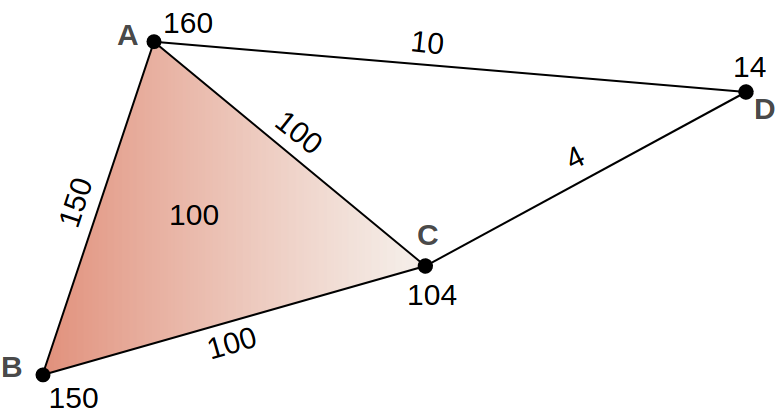
\includegraphics[height=2.3cm]{./figures/cc1.png}}%
\settowidth{\tempwidth}{\usebox{\tempbox}}%
\hfil\begin{minipage}[b]{\tempwidth}%
\raisebox{-\height}{\usebox{\tempbox}}%
\scriptsize{\captionof*{figure}{(b) Co-authorship complex}}%
\label{fig:co-authoship-complex}%
\end{minipage}%
\vspace{5pt}
%\end{table*}
\savebox{\tempbox}{\scriptsize{
\begin{blockarray}{cccccc}
\tiny{AB} & \tiny{AC} & \tiny{AD} & \tiny{BC} & \tiny{CD} \\
\begin{block}{(ccccc)c}
  3 & 0 & 1 & 0 & 0 & \tiny{AB} \\
  0 & 3 & 1 & 0 & -1 & \tiny{AC} \\
  1 & 1 & 2 & 0 & 1 & \tiny{AD} \\
  0 & 0 & 0 & 3 & -1 & \tiny{BC}\\
  0 & -1 & 1 & -1 & 2 & \tiny{CD}\\
\end{block}
\end{blockarray}}}%
\settowidth{\tempwidth}{\usebox{\tempbox}}%
\hfil\begin{minipage}[b]{\tempwidth}%
\raisebox{-\height}{\usebox{\tempbox}}%
\scriptsize{\captionof*{figure}{(c) $1$-Laplacian}}%
\end{minipage}%
%\end{table*}
\caption{Example of co-authorship complex and its $1$-Laplacian build from data}\label{fig:data2complex}
\end{figure}

\subsection{Simplicial Laplacians}
We are in this paper concerned with finite simplicial complexes. In particular, it is not necessary for them to come equipped with some embedding into Euclidean space, nor do we demand that they triangulates a Riemannian manifold. To define a discrete version of the Laplacian for simplicial complexes, one simply takes the linear adjoint of the coboundary operator with respect to the inner product, defining $\delta_i^\ast:C^{i+1}\to C^i$ by
\begin{align*}
  \ip{\delta_i f_1}{f_2}_{i+1} =\ip{f_1}{\delta_i^\ast f_2}_{i} \quad \forall f_1\in C^{i}(K), f_2 \in C^{i+1}(K).
\end{align*}
In analogy with Hodge--de Rham theory~\cite{madsen1997calculus}, we then define the \emph{degree-$i$ simplicial Laplacian} of a simplicial complex $K$ as the linear operator $\lap_i:C^i(K)\to C_i(K)$ such that
\begin{equation*}
  \lap_i = \lapu_i + \lapd_i,\\
\end{equation*}
where $\lapu_i =  \delta_{i}^\ast\circ\delta_{i}$ and $\lapd_i = \delta_{i-1}\circ\delta_{i-1}^\ast$. In case $i=0$, $\mathcal{L}_0$ corresponds to the classical graph Laplacian. Observe that there are $p$ Laplacians for a complex of dimension $p$. In most practical applications, the matrices for the Laplacians are very sparse and can easily be computed as a product of sparse coboundary matrices and their transposes. Since the Laplacians encode information about the adjacency of the simplices, they can be interpreted as a message passing functions. Additionaly, the carry valuable topological information about the simplicial complex. In particular, Eckmann \cite{eckmann1944} proved that the kernel of the $k$-Laplacian is isomorphic to the $k$-(co)homology of its associated simplicial complex. In other words, the number of zero-eigenvalues tells us the number of $k$-dimensional holes. For a more detailed introduction on this topic we refer the reader to~\cite{horak2013spectra}.
\subsection{Simplicial Neural Networks}
Our contribution is a notion of convolution for simplicial complexes using the Laplacian.


\begin{itemize}
\item Goal: building a convolutional NN whose input is an arbitrary $p$-cochain on a fixed simplicial ocmplex $K$
\item  Definition of Fourier Transform
\item Convolutional Filters: low degree polynomials in the frequency domain
\item Implemented using Chebyshev polynomials
\item Computational cost: good the $p$-Laplacian is localized and sparse.
\item FIX ME
\item FIX ME
\item FIX ME
\item FIX ME
\item FIX ME
\item FIX ME
\item FIX ME
\item FIX ME
\item FIX ME
\item FIX ME
\item FIX ME
\item FIX ME
\item FIX ME
\item FIX ME
\end{itemize}

\begin{figure}[htbp]
  \centering

\includegraphics[width=5cm]{example-image-golden}
  \caption{Maybe figures SNN} \label{fig:SNN}
\end{figure}